\documentclass[english]{his-thesis}

% Import user's metadata such as title, name, ISBN, ...
\usepackage{hismetadata}
\title{Game-calibrated and user-tailored remote detection of emotions}
\subtitle{A non-intrusive, multifactorial camera-based approach for detecting stress and boredom of players in games}
\subject{Informatics}
\date{1970}{4}{31}
\isbn{979-123-456-789}
\seriesnumber{42}
\author{Fernando Bevilacqua}
\decidedby{den internationella kommittéen för den fjärde internationalen}
\defensedaytimeroom{mån}{15}{april}{2016}{16.15}{Portalen, våning~5}
\opponent{K. Blaubär, Salzburg University}
%% \dissertationtype is the official name of the publication's
%% type, either in Swedish or English (whatever applies to you).
%% The value set here is used among others on the title page.
%% Not to be mixed up with \publicationtype
% \dissertationtype{licentiatexamen}
\dissertationtype{filosofie doktorsexamen}
\dissertationarea{informationsteknologi}
\spokenlanguage{engelska}
%\spokenlanguage{svenska}
%% \publicationtype controls whether the document is a
%% dissertation or a licentiate thesis. It has to be one
%% of the two values. It determines various formatting
%% aspects, such as the default colors (purple vs. grey).
%% Not to be mixed up with \dissertationtype
\publicationtype{dissertation}% or \publicationtype{licentiate}

% Import functionality for a purple title page
\usepackage{histitlepage}
% Import functionality to set bibliography
\usepackage{hisbibliography}
% Some example bibliography
\addbibresource{references.bib}
% Import functionality for text formatting
\usepackage{histextformatting}
% Import functionality for "own publications" page
\usepackage{hisownpublications}


% For generating dummy text.
% Only necessary for the example document, remove for "real dissertations"
\hyphenation{vesti-bulum sce-leris-que}

\begin{document}
% set default font to Georgia 9.5pt
\fontgeorgia{9.5}{11}

\maketitle

\cleardoublepage
\pagenumbering{roman}% Switch to Roman page numbers
\setcounter{page}{1}% Start page numbers from 'i' (Roman 1)
\pagestyle{headings}

%\chapter*{Abstract}

Questionnaires and physiological measurements are the most common approach used to obtain data for emotion estimation in the field of human-computer interaction (HCI) and games research. Both approaches interfere with the natural behavior of users, which affects any research procedure. Initiatives based on computer vision and remote extraction of user signals for emotion estimation exist, however they are limited. Experiments of such initiatives were performed under extremely controlled situations with few game-related stimuli. Users had a passive role with limited possibilities for interaction or emotional involvement, differently than game-based emotion stimuli, where users take an active role in the process, making decision and directly interacting with the media. Previous works also focus on predictive models based on a group perspective. As a consequece, a model is usually trained from data of several users, which in practice describes the average behavior of the group, excluding or diluting key individualities of each user. In that light, there is a lack of initiatives focusing on non-obtrusive, user-tailored emotion detection models, in particular regarding stress and boredom, within the context of games research that are based on emotion data generated from game stimuli.

This thesis proposal presents a research that aims to fill that gap, providing the HCI and the games research community with an emotion detection process, instantiated as a software tool, which can be used to remotely study users emotions in a non-obtrusive way within the context of games. The main knowledge contribution of this research is a novel process for emotion detection that is remote (non-contact) and constructed from a game-based, multifactorial, user-tailored calibration phase. The process relies on computer vision and remote photoplethysmography (rPPG) to read user signals, e.g. heart rate and facial actions, without physical contact during the interaction with games in order to perform the detection of stress/boredom levels of users. The approach is automated and does not require specialized equipment, e.g. sensors, only a regular video camera.

Current results of this research show that individualities can be detected regarding facial activity, e.g. increased number of facial actions during the stressful part of games. Regarding physiological signals, findings are aligned with and reinforce previous research that indicate higher HR mean during stressful situations in a gaming context. The findings also suggest that changes in the HR during gaming sessions is a promising indicator of stress, which can be incorporated into a model aimed at emotion detection. The literature reviews, the experiments conducted so far and the planned future tasks support the idea of using a set of signals, e.g. facial activity, body movement, and HR estimations as sources of information in a multifactorial analysis for the identification of stress and boredom in games. It will produce a novel user-tailored approach for emotion detection focused on the behavioral particularities of each user instead of the average group pattern. The proposed approach will be implemented as a software tool, which can be used by researchers and practitioners for games research.

%\chapter*{Summary}

Summary

%\chapter*{Acknowledgements}

Acknowledgements


\ownpublications[Some optional text here]{Walley2000,landis1977measureobserveragreement,henkel2006revealingemblinux}{knauth2003prevcompmeasuresshiftwrk,yang2010wikipediacontrib,dedrick2006scope}

\tableofcontents
\listoffigures
\listoftables

\cleardoublepage
\pagenumbering{arabic}% Switch to Arabic page numbers
\setcounter{page}{1}% Start page numbers from '1'
\pagestyle{headings}

%\chapter{Introduction}
\label{c:introduction}

In human-computer interaction (HCI) research, the study of the relation between users and systems is of interest. Within the context of games research in particular, the relation between the player and the game is an important topic. Such relation comprehends concepts as engagement and immersion \parencite{boyle2012engagement} and the investigation of the elements that influence those concepts.

To perform such investigations, researchers need to rely on methods that are able to capture the user's emotional state within the proposed context. The most commonly used techniques to obtain data regarding emotional states of players in a game are self-reports (questionnaires) and physiological measurements \parencite{mekler2014systematic}. Questionnaires are practical and ease to use tools, however they require a shift in attention, hence breaking or affecting the level of engagement/immersion of the user. Physiological signals, on the other hand, have been used to obtain information from users without causing interruptions \parencite{bousefsaf2013remote,yun2009game,rani2006empirical,tijs2008dynamic}. Sensors, despite avoiding interruptions, are usually perceived as uncomfortable and intrusive, since they require the proper setup in the person's body. Additionally sensors might restrict player's motion abilities, e.g. a sensor attached to a finger prevents the use of that finger. Sensors also increase user's awareness of being monitored \parencite{yamakoshi2007preliminary,yamaguchi2006evaluation,healey2005detecting}, which disturbs the results of an investigation.

%Questionnaires, however, require the user to stop the game activity in order to share his/her current state. The frequency that such questionnaires are issued is also a concern. If performed too often, more information might be collected, but the data might contain noise caused by the frequent interruptions, e.g. player is more stressed/bored by the questionnaire interruptions than by the game itself. If performed too sparse, not enough information will be gathered from the player.

Despite the mentioned problems, sensors continue to be used because there is a significant amount of information that can be read from the human body, such as heart rate (HR), respiratory rate (RR), facial expressions, among others. The information provenient from the human body can be seen as input signals for emotion estimation. The process of mapping such signals to an emotional state, however, is a significant task. It involves testing/defining what are the possible emotional states a person can experience \parencite{mandryk2006continuous}, as well as comparing which signals are better predictors of such states \parencite{jerritta2011physiological}. A number of studies \parencite{kukolja2014comparative} suggest that the analysis of a combination of different input signals, known as multimodal analysis, is more likely to produce accurate results when mapping emotional states. The mapping process itself is another important part of the equation that influences the results.

Research in different areas, such as affective computing and computer vision, aim to improve the workflow of emotion investigation with non-obtrusive approaches involving the aforementioned signals. By using computer vision and a video stream captured by a camera, one can obtain different information from a subject, such as facial expressions and physiological signals, without the use of physical sensors.

\section{Problem specification}

As previosly described, questionnaires and physiological measurements are the most common approach used to obtain data for emotion estimation. Both approaches interfere with the natural behavior of users, which affects any research procedure. Initiaties based on computer vision and remote extraction of user signals for emotion estimation are feasible. The remote detection of HR, for instance, proved a promising approach to infer boredom/stress levels \parencite{kukolja2014comparative} or cognitive stress \parencite{mcduff2014remote} of a person. Experiments regarding such approaches, however, were performed under extremely controlled situations with few game-related stimuli. A significant limitation of such approaches was that subjects were asked to remain still during the experiment. This is an uncommon user behavior during the interaction with emotional estimulators that hinders the real efficiency of such remote detection techniques. Users are likely to behave in a more natural way, e.g. featuring facial expressions and moving the body, which directly affect the remote measurements of physiological signals.

Another problem is that subjects had limited interaction with the content being presented: they performed tasks mentally (e.g. counting), watched videos/images or performed gamified cognitive tests for a short period of time. Those are artificial situations that are unlikely to happen in real-life situations, especially in a gaming session with a challenging game lasting for several minutes. In that situation, the subject will probably move and present variations of facial actions during the gaming session \parencite{bevilacqua2016variations}. With game-based emotion stimuli, users take an active role in the process, making decision and directly interacting with the media. When images, videos or gamified tests are employed, users take a passive role with limited possibilities for interaction or emotional involvement. In addition to the limited use of game-related stimuli for emotion elicitation, previous works focus on predictive models based on a collective perspective. As a consequece, a model is usually trained from data of several users, which in practice describes the average behavior of the group, excluding key individualities of each user.

In that light, there is a lack of initiatives focusing on non-obtrusive, user-tailored emotion detection models, in particular regarding stress and boredom, within the context of games research that are based on emotion data generated from game stimuli. This thesis presents a research that aims to fill that gap, providing the HCI and the games research community with tools to remotely study users emotions in a non-obtrusive way within the context of games.

\section{Research aim}

This research presents an approach for remotely detecting and measuring the changes in stress and boredom levels of a player during the interaction with a game. The process is based on a non-contact, multifactorial analysis of user signals, e.g. HR and facial expressions, obtained from a video stream. The foundation is based on the construction of a user-tailored model, built on information obtained from the user while he/she played a set of calibration games. The model uses the remotely obtained signals from the user in conjunction with the calibration data to detect the player's changes regarding stress and boredom levels in any other game.

%According to previous research, the use of games as a emotional triggering mechanism is a feasible approach. Additionally an user-tailored model is a more efficient approach than a group-tailored model for the detection of emotional changes in users.

\section{Contributions}

This research presents a method that is able to interpret remotely acquired signals from a person and detect his/her current emotional state regarding stress and boredom according to data obtained from a calibration phase. The result adds to the body of knowledge of HCI and games research. The main contribution is a method for remote acquisition and analysis of physiological and non-physiological signals of a player in order to detect the stress and boredom levels of that player.

A purely remote-based approach, as the one proposed by this research, enhances the tooling available regarding investigation methods of stress and boredom. The approach, which is based on calibration games, maps a set of variations of signals into two specific emotional states (stress/boredom). This information can be used by other researchers to identify important moments during the interaction of players with games, such as when the recognized pattern is closer to stress. In game design research, for instance, that instrumentation can be used as another way of obtaining information from a user during a game session. The use of questionnaires, which shift the player's focus away from the game, can be enhanced and/or replaced by the use of the proposed method, making the process less obtrusive. By remotely reading information regarding stress and boredom, a researcher can use such information to better understand concepts as engagement, frustration, immersion and flow in games, for instance. Additionally it can be used in any activity that relies on stress/boredom as an important measurement, such as usability tests in software and games, for instance. Another contribution is a better understanding of how the selected signals are related to stress/boredom. Other researchers might use that information in contexts outside the games area, such as the measurement of costumers satisfaction or interest in stores.

%The proposed method will be based on the analysis of the variation of signals of a person according to a reference (calibration data). This approach is significantly different from the already existing methods, which focus on training a model to detect pre-defined states (e.g. stress, boredom, rest) based on the current value of the acquired signals. The foundation of the approach proposed in this research is the use of variations, which by nature account for differences between the current state and any other known state (the calibration profile, for instance). This configuration allows the method to be expanded or further investigated to produce a scale regarding the measurement of stress and boredom. Different from a direct mapping of signals to a state, a scaled measurement might inform the researcher of how much stress or boredom the player is experiencing, as opposed to just informing he/she is stressed or bored. This might be possible to be achieved with a machine learning model, for instance, but it will require a complex training setup. which will inevitably result in frequent interruptions of the player for collecting self-reported stress/boredom levels. This will disturb immersion/engagement with the game, probably resulting in noise in the mapping.

%A researcher is be able to increase the internal validity of his/her workflow by ensuring the player keeps the focus on the game without interruptions and by minimizing the side effects (and inconveniences) of physical monitoring. This research can also be deployed as a solution for game developer studios to automatically analyze hours of recorded gameplay and highlight the moments when boredom/stress levels changed significantly. As a complement the solution is based on a single, ordinary camera and a software implementation, which eliminates the use of complex setups of physical sensors. It eases the investigation process and reduces costs.

\section{Thesis overview and structure}

%\chapter{Research methodology}

The aim of this research is to produce a technology-based solution to the problem of non-contact emotion detection within the context of games research. The solution is a software composed of a user-tailored model that is trained from a game-based calibration phase and is able to infer the emotional state of a player regarding stress and boredom via analysis of remotely acquired user signals. The contructs, models and methods involved in such aim have been individually studied in previous research, however the combination of all those elements in a single solution within the context of games research is novel. The utilization of those elements in combination is not yet proved to work, so an iterative and incremental process must be conducted to identify challenges, problems and solutions to achieve the desired goal.

\begin{figure}[h]
    \centering
    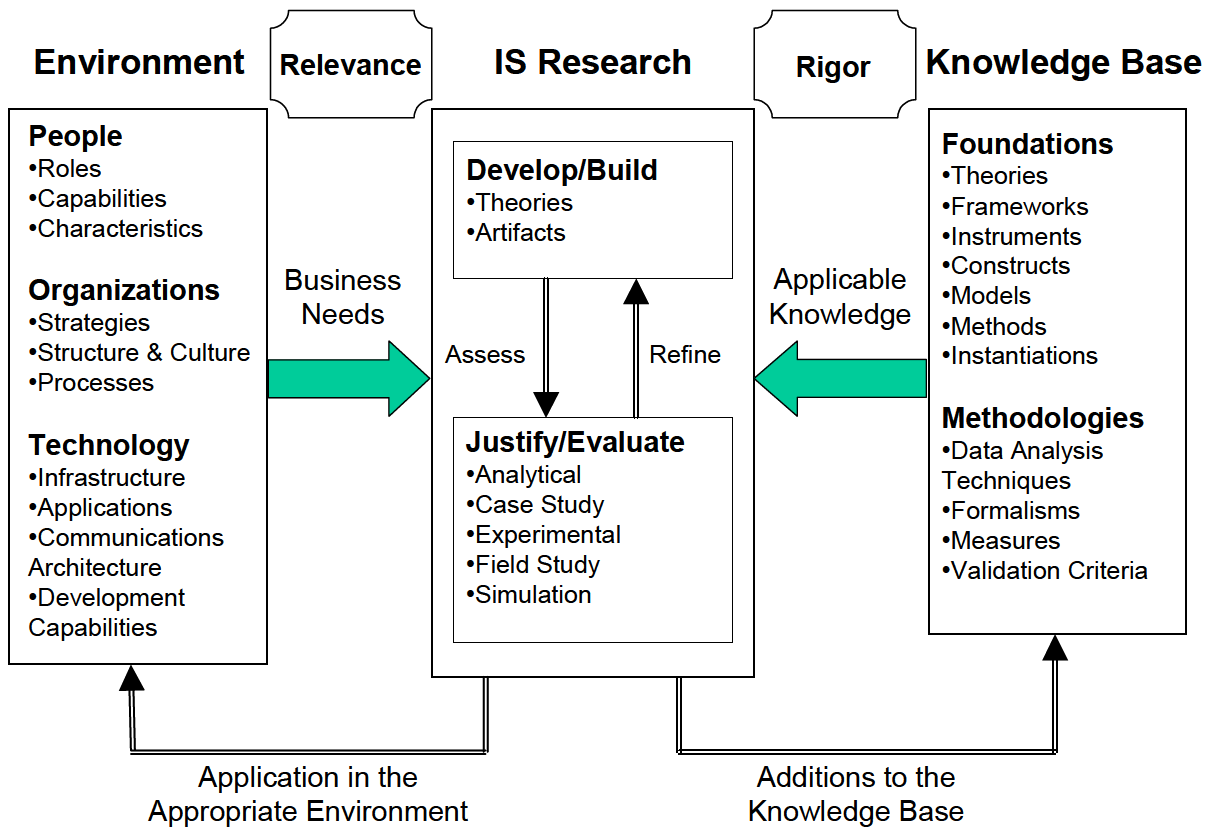
\includegraphics[width=\textwidth]{figures/hevner-research-framework.png}
    \caption{A framework for design science in the context of Information Technology \parencite{hevner2004design}}
    \label{fig:hevner-research-framework}
\end{figure}

A research methodology that fits such iterative process is design science. As defined by \textcite{hevner2004design} and illustrated in Figure \ref{fig:hevner-research-framework}, design science is a problem solving process that explores a relevant problem within an environment, iteratively measuring and refining the proposed solution according to the existing body of knowledge. The progress is made iteratively as the scope of the design of the artifact is expanded based on the discovery of available means, ends and constraints.

The use of a game-based calibration phase in this research influences how users behave during the emotion elitication process, e.g. body movement and facial expression. The movement of users directly impact the techniques for remote extraction of user signals during both the calibration phase and the emotion estimation phase, since those techniques are highly influenced by motion. The accuracy of those techniques regarding the remotely acquired signals is affected as well, which might invalidate the feasibility of remotely reading determined physiological and non-physiological signals required by the emotion estimaion model. The computer vision techniques, the model and the process associated with them must be continuously investigated and adapted to overcome those challenges. As a consequence, an iteractive cycle of development and research is required, as illustrated by Figure \ref{fig:hevner-generate-test}. In each iteration, a possible solution for the current set of problems is generated, rigourly tested and evaluated, producing information to guide the next iterations in the cycle. The set of design alternatives in this research are related to the identification of physiological and non-physiological signals to be used in the emotion detection process, how they can be elicitated with games in a calibration phase, which computer vision techniques can be employed to remotely acquire the signals and which machine learning model is able to map the information into emotional states. The set of constraints involve problems associated with users behaving naturally, e.g. laughing and moving the body during the procedure, use of non-specialized hardware, e.g. ordinary camera, accuracy and efficienty of the solution, among others.

\begin{figure}[h]
    \centering
    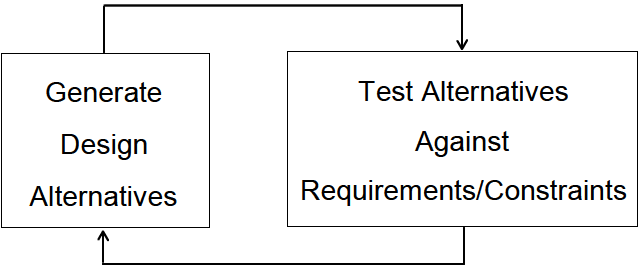
\includegraphics[width=0.6\textwidth]{figures/hevner-generate-test.png}
    \caption{The Generate/Test cycle. Adapted from \textcite{hevner2004design}}
    \label{fig:hevner-generate-test}
\end{figure}

%The aim of this research is to produce a utility tool, i.e. software, which is an artifact based on a model built on existing theories, which will be combined in a new and innovative way. Since the result of the research is a model, which will be built from different measurements to predict or infer a state, the present work stands on the positivism paradigm. Essentially this work will formulate a theory about how the variation of physiological signals relate to stress/boredom levels in the context of games and how it can be remotely detected. The involvement of humans in the process might relate to the social side of interpretivism, however the foundation of the work is still based on the analysis of physiological signals. Such signals and their patterns might be different for each person, however they are still ordered and regular under the human being perspective. As a consequence, they can be objectively observed, measured and analysed with a quantitative approach and hypothesis testing.

Design-science research requires the application of rigorous methods in both the construction and evaluation of the designed artifact \parencite{hevner2004design}. One of such evaluation methods is experimental research, which is the strategy used to build and validate the knowledge in this project. Such approach is composed of a set of research designs that use controlled testing and manipulation of variables in order to understand causal processes. The foundation of an experiment is to manipulate a variable (or a set of them) and measure any changes in other variables. It establishes the effect on a dependent variable, which is the focus of the research. The model being constructed in this research links the variations of user signals to stress/boredom levels in the context of games, hence there is a causal effect in the process since identified variations (cause) will precede changes in stress/boredom levels (effect). It progresses to the construction of a hypothesis where the cause will consistently lead to the same effect so the link between variations of signals and emotional levels can be inferred or predicted.

Each iteration in the design of the artifact will be constructed based on systematical investigation of existing theories, which will be refined and adapted to the context of the artifact. An experiment will validade the current artifact, producing information to guide the next iteration. The following section detail what is the current state of the project.

%\section{Research objectives}

%The objective of this research is to produce a method that is able to interpret remotely acquired signals from a person playing a game and detect his/her current emotional state regarding stress and boredom according to data previously obtained in a calibration phase. The model will be implemented in a software that uses a video feed to detect the person's emotional state.

%The current approaches used to obtain information from the players during games research inevitably affect the player's experience. They require the user to stop the game activity in order to share his/her current state, such as by answering a questionnaire. The frequency that such questionnaires are issued is also a concern. If performed too often, more information might be collected, but the data might contain noise caused by the frequent interruptions, e.g. player is more stressed/bored by the questionnaire interruptions than by the game itself. If performed too sparse, not enough information will be gathered from the player. A physical sensor attached to a player, on the contrary, allows a continuous monitoring process, however it is intrusive and might interfere with the player capacity to interact with the game. It might prevent the use or movement of specific parts of the body, for instance. Physical sensors also increase the chances of the player to behave differently as a side-effect of the monitoring process itself.

%A purely remote-based solution, as the one proposed by this research, enhances the tooling available to the games research community regarding investigation methods of stress and boredom. A games researcher will be able to increase the internal validity of his/her workflow by ensuring the player keeps the focus on the game without interruptions and by minimizing the side effects (and inconveniences) of physical monitoring. This research could also be deployed as a solution for game developer studios to automatically analyze hours of recorded gameplay and highlight the moments when boredom/stress levels changed significantly. As a complement the solution will be based on a single, ordinary camera and a software implementation, which eliminates the use of complex setups of physical sensors. It eases the investigation process and reduces costs.

\section{Current state of research}

As previously mentioned, this research is based on an interative problem solving strategy that involves the investigation and evaluation of different components. Figures \ref{fig:user-tailored-calibration} and \ref{fig:user-tailored-use}, in section \ref{sec:research-aim}, illustrate the combined use of the different parts involved in this project, which are all connected to the research objectives presented in section \ref{sec:contributions}. Figure \ref{fig:components-objectives} illustrates the correlation among the research objetives and the parts required to achieve the proposed research aim.

\begin{figure}[h]
    \centering
    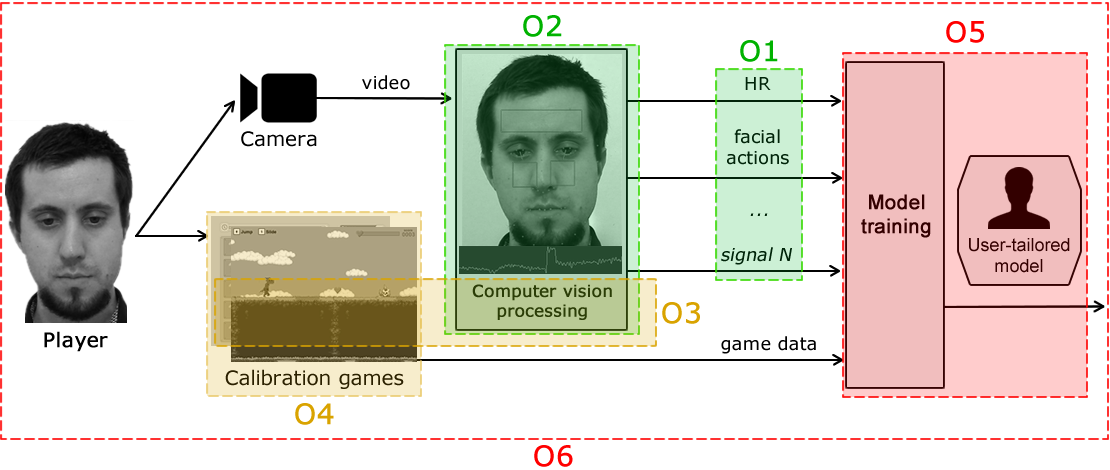
\includegraphics[width=\textwidth]{figures/components-objectives.png}
    \caption{Correlation among the research objetives and the parts required to achieve the proposed research aim. Red labels: not fulfilled yet. Yellow labels: partially fulfilled. Green labels: completely fulfilled.}
    \label{fig:components-objectives}
\end{figure}

Objectives marked in red and yellow are not fulfilled and partially fulfilled, respectively, so more investigation will be conducted regarding them. For information regarding future work, refer to chapter \ref{ch:closing}. Objectives marked in green have been completely fulfilled and the theories, concepts and results associated to each of them is documented in this thesis proposal. The chapters where such documentation and the associated objectives exist in this thesis proposal is presented in Figure \ref{fig:research-current-state}.

%The experiment design will be based on a within-subject approach \cite{lane2015online}. In such approach, all participants perform at all levels of the treatment and there are no control groups. It is the opposite of a between-subjects approach, where subjects are divided in more than one group that receive different treatments. In that approach there are special groups, called control groups, that receive no treatment. The comparison between the control groups and the treatment groups ensures internal validity. In the context of this research, physiological signals will be measured, so the division of subjects into more than one group poses a comparison problem. Each individual will inevitably differ from one another regarding physiological signals, such as variations in average HR during rest, for instance. When measuring HR, for instance, some subjects will have higher/lower HR mean than others, independent of the group they are in or the treatment they undergo. To counter that problem, the experiment will use a one-group posttest design \cite{kirk1982experimental}, as illustrated by Figure \ref{fig:experiment}. Using the first row as an example, subject $S_0$ played game $G_a$ as the first level of the treatment, followed by a post-test of that game ($PT_a$), then a rest period. In the second level of the treatment, the subject played game $G_b$, followed by a post-test of that game ($PT_b$), then another rest period. Finally in the third level of the treatment, the subject played game $G_c$ followed by a post-test of that game ($PT_c$).

%\begin{figure}[ht]
%    \centering
%    \includegraphics[scale=0.5]{imgs/experiment-design.png}
%    \caption{One-group posttest experiment design used in this research. $S_j$ represents the $j^{\text{th}}$ subject, $G_i$ represents a game of type $i$, $PT_i$ is the post-test for game $G_i$ and $rest$ is a resting period.}
%    \label{fig:experiment}
%\end{figure}

%By using a one-group posttest design, each individual will perform on all levels of the treatment (play a set of different games). The within-subjects approach ensures that the differences between subjects are not interfering in the comparison, since a subject is being compared to his/herself in the different levels of the treatment. Subjects are not being compared among each other. In essence, each subject is serving as his/her own control group. According to Kirk \cite{kirk1982experimental}, the one-group posttest design should only be used when the researcher knows the mean value of the independent variable when no treatment is in effect. Such information will be obtained during the resting periods of the experiment, where the baseline value for all measured signals can be established for each subject.

%The process of sampling a group of participants for each experiment will follow the convenience sampling approach, a non-probability sampling technique where participants are recruited because of their convenient accessibility/proximity to the researcher. Volunteers will be randomly recruited for each experiment. A probability sampling approach, where each individual of the population has an equal chance of being selected, would be ideal and would strength the external validity of the research. However the costs, logistics and time constraints associated with it makes such approach impractical in the context of this research.

Both objectives \textbf{O1} and \textbf{O2} have already been fulfilled. After the first literature review, the accomplishment of \textbf{O1} produced the identification of the main concepts, theories and signals associated with phychophysiological profile of users and their emotions. Chapters \ref{ch:literature-games}, \ref{ch:literature-physiological} and \ref{ch:literature-multifactorial} present the results of such literature review. The results of the literature review regarding objective \textbf{O2}, which focus on the identification of existing computer vision techniques to remotely extract signals from users, is presented in chapters \ref{ch:literature-face} and \ref{ch:literature-rppg}. The investigation also produced a publication regarding emotion detection and remote measurement of physiological signals \parencite{bevilacqua2015proposal}.

\begin{figure}[ht]
    \centering
    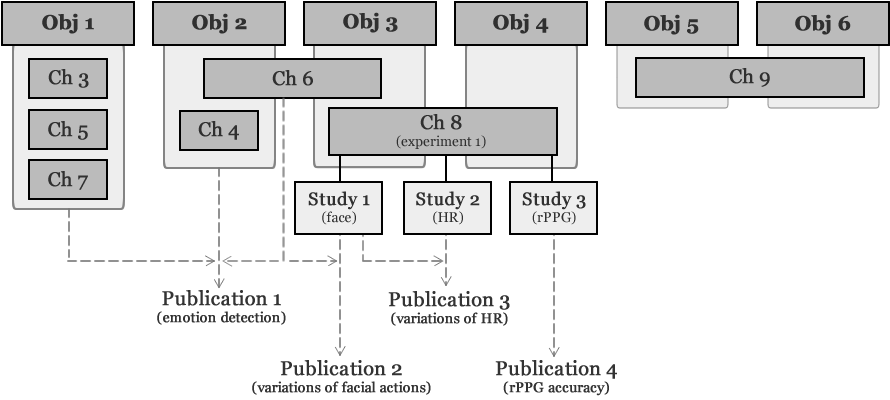
\includegraphics[width=\textwidth]{figures/research-current-state.png}
    \caption{The thesis proposal chapters coupled with the research objetives they cover.}
    \label{fig:research-current-state}
\end{figure}

Objective \textbf{O3} is being finalized. The aim of that objective, which is the investigation of feasibility, accuracy and challenges regarding the application of computer vision techniques within the context of games, was performed as an experiment. The experiment and the three studies conducted on the collected data are described and presented in chapter \ref{ch:experiment1}. Each one of those studies resulted in a publication, which present results regarding variations of facial actions \parencite{bevilacqua2016variations}, variations of heart rate \parencite{bevilacqua2017changes} and accuracy evaluation of the selected computer vision technique \parencite{bevilacqua2017accuracy}. The last two aforementioned publications were recently submitted for review. The main challenges regarding the application of the computer vision techniques within the context of games have already been identified. A publication \parencite{bevilacqua2017accuracy} and the literature review presented in chapter \ref{ch:literature-rppg} show the limitations of the computer vision technique when applied to contexts of games research involving natural behavior of users, e.g. head movement and face oclusion. A new study will be conducted to investigate ways to improve the computer vision technique to eliminate or mitigate such limitations.

Objective \textbf{O4} has been partially fulfilled. A pilot study, an experiment (described in chapter \ref{ch:experiment1}) and two publications \parencite{bevilacqua2016variations,bevilacqua2017changes} describe and validate the concept of calibration games. Up to the present moment, however, the variation of the signals produced by such calibration games have not been employed in any studies or experiments involving emotion detection, so its utility within the context of this research needs to be further investigated.

The future work planed to fullfil all research objectives is described in chapter \ref{ch:closing}.

%\chapter{Conclusion}
\label{ch:conclusion}

Questionnaires and physiological measurements are the most common approach used to obtain data for emotion estimation in the field of HCI and games research. Both approaches interfere with the natural behavior of users, which affects any research procedure. Initiatives based on computer vision and remote extraction of user signals for emotion estimation exist, however they are limited. Experiments of such initiatives were performed under extremely controlled situations with few game-related stimuli. Users had a passive role with limited possibilities for interaction or emotional involvement, differently than game-based emotion stimuli, where users take an active role in the process, making decision and directly interacting with the media. Previous works also focus on predictive models based on a group perspective. As a consequece, a model is usually trained from data of several users, which in practice describes the average behavior of the group, excluding or diluting key individualities of each user. In that light, there is a lack of initiatives focusing on non-obtrusive, user-tailored emotion detection models, in particular regarding stress and boredom, within the context of games research that are based on emotion data generated from game stimuli.

This thesis proposal presented a research that aims to fill that gap, providing the HCI and the games research community with an emotion detection process, instantiated as a software tool, which can be used to remotely study users emotions in a non-obtrusive way within the context of games. Current results of this research show that individualities can be detected regarding facial activity, e.g. increased number of facial actions during the stressful part of games. Regarding physiological signals, findings are aligned with and reinforce previous research that indicate higher HR mean during stressful situations in a gaming context. The findings also suggest that changes in the HR during gaming sessions is a promising indicator of stress, which can be incorporated into a model aimed at emotion detection. As pointed out by previous work, a user-tailored model based on several signals, e.g. HR and facial activity, is more likely to detect emotional states of users.

The literature reviews, the experiments conducted so far and the planned future tasks support the idea of using a set of signals, e.g. facial activity, body movement, and HR estimations as sources of information in a multifactorial analysis for the identification of stress and boredom in games. It will produce a user-tailored approach for emotion detection focused on the behavioral particularities of each user instead of the average group pattern.

%\begin{appendix}
\chapter{How I Got My Appendix Removed}
\end{appendix}


\chapter{Introduction}
  \section{Motivation}
  \section{Problem specification}
  \section{Contributions}
  \section{Thesis overview and structure}

\chapter{Literature review}
  \section{Introduction}
  \section{Emotions}
    \subsection{Russell's AV dimensional theory of emotions}
    \subsection{Theory of flow}
  \section{Games and emotions}
    \subsection{Stress, boredom and flow}
    \subsection{Immersion, engagement and sense of presence}
  \section{Emotions and facial analysis}
    \subsection{Facial features and emotion detection}
    \subsection{Emotion detection based on facial movement}
  \section{Emotions and physiological signals}
    \subsection{Physiology of heart rate}
    \subsection{Heart rate, stress and frustration}
  \section{Remote photoplethysmography}
    \subsection{Introduction}
    \subsection{Structure of an rPPG technique}
      \subsubsection{Signal extraction}
      \subsubsection{Signal estimation}
      \subsubsection{Heart rate estimation}
    \subsection{rPPG techniques}
    \subsection{Accuracy and limitations}
      \subsubsection{Sampling frequency and estimation error}
      \subsubsection{Natural behavior and accuracy}
    \subsection{Emotion estimation}
  \section{Multifactorial emotion estimation}

\chapter{Variations of Facial actions during a gaming session}
  \section{Introduction}
  \section{Data and methods}
    \subsection{Participants, Materials and Procedures}
    \subsection{Games and stimuli elicitation}
    \subsection{Classification analysis}
  \section{Results and discussions}
  \section{Conclusions}

\chapter{Changes in heart rate during a gaming session}
  \section{Introduction}
  \section{Data and methods}
    \subsection{Participants, Materials and Procedures}
    \subsectioxzn{Analysis}
  \section{Results and discussions}
  \section{Conclusions}

\chapter{Accuracy of rPPG measurements applied to gaming sessions with natural behavior}
  \section{Introduction}
  \section{Data and methods}
    \subsection{Participants, Materials and Procedures}
    \subsection{Implementation of the rPPG technique}
    \subsection{Analysis}
  \section{Results and discussions}
  \section{Conclusions}

\chapter{Closing remarks}
  \section{Conclusion}
  \section{Future work}


\begin{fullarticles}
%\fullarticle{bergmarklund2013gamesformaleducationalsettings}{manual.pdf}
\end{fullarticles}

% from package 'hisbibliography'
\listofreferences

% from package 'hisbibliography'
\dissertationlist

\end{document}
